\documentclass[10pt, a5paper]{article}
\usepackage{pdfpages}
\usepackage{parallel}
\usepackage[T2A]{fontenc}
\usepackage{ucs}
\usepackage[utf8x]{inputenc}
\usepackage[polish,english,russian]{babel}
\usepackage{hyperref}
\usepackage{rotating}
\usepackage[inner=2cm,top=1.8cm,outer=2cm,bottom=2.3cm,nohead]{geometry}
\usepackage{listings}
\usepackage{graphicx}
\usepackage{wrapfig}
\usepackage{longtable}
\usepackage{indentfirst}
\usepackage{array}
\newcolumntype{P}[1]{>{\raggedright\arraybackslash}p{#1}}
\frenchspacing
\usepackage{fixltx2e} %text sub- and superscripts
\usepackage{icomma} % коскі ў матэматычным рэжыме
\PreloadUnicodePage{4}

\newcommand{\longpage}{\enlargethispage{\baselineskip}}
\newcommand{\shortpage}{\enlargethispage{-\baselineskip}}

\def\switchlang#1{\expandafter\csname switchlang#1\endcsname}
\def\switchlangbe{
\let\saverefname=\refname%
\def\refname{Літаратура}%
\def\figurename{Іл.}%
}
\def\switchlangen{
\let\saverefname=\refname%
\def\refname{References}%
\def\figurename{Fig.}%
}
\def\switchlangru{
\let\saverefname=\refname%
\let\savefigurename=\figurename%
\def\refname{Литература}%
\def\figurename{Рис.}%
}

\hyphenation{admi-ni-stra-tive}
\hyphenation{ex-pe-ri-ence}
\hyphenation{fle-xi-bi-li-ty}
\hyphenation{Py-thon}
\hyphenation{ma-the-ma-ti-cal}
\hyphenation{re-ported}
\hyphenation{imp-le-menta-tions}
\hyphenation{pro-vides}
\hyphenation{en-gi-neering}
\hyphenation{com-pa-ti-bi-li-ty}
\hyphenation{im-pos-sible}
\hyphenation{desk-top}
\hyphenation{elec-tro-nic}
\hyphenation{com-pa-ny}
\hyphenation{de-ve-lop-ment}
\hyphenation{de-ve-loping}
\hyphenation{de-ve-lop}
\hyphenation{da-ta-ba-se}
\hyphenation{plat-forms}
\hyphenation{or-ga-ni-za-tion}
\hyphenation{pro-gramming}
\hyphenation{in-stru-ments}
\hyphenation{Li-nux}
\hyphenation{sour-ce}
\hyphenation{en-vi-ron-ment}
\hyphenation{Te-le-pathy}
\hyphenation{Li-nux-ov-ka}
\hyphenation{Open-BSD}
\hyphenation{Free-BSD}
\hyphenation{men-ti-on-ed}
\hyphenation{app-li-ca-tion}

\def\progref!#1!{\texttt{#1}}
\renewcommand{\arraystretch}{2} %Іначай формулы ў матрыцы зліпаюцца з лініямі
\usepackage{array}

\def\interview #1 (#2), #3, #4, #5\par{

\section[#1, #3, #4]{#1 -- #3, #4}
\def\qname{LVEE}
\def\aname{#1}
\def\q ##1\par{{\noindent \bf \qname: ##1 }\par}
\def\a{{\noindent \bf \aname: } \def\qname{L}\def\aname{#2}}
}

\def\interview* #1 (#2), #3, #4, #5\par{

\section*{#1\\{\small\rm #3, #4. #5}}

\def\qname{LVEE}
\def\aname{#1}
\def\q ##1\par{{\noindent \bf \qname: ##1 }\par}
\def\a{{\noindent \bf \aname: } \def\qname{L}\def\aname{#2}}
}

\switchlang{en}
\begin{document}
\title{Case Study: Parallel Programming in Python with COMPSs}
\author{Nikolay Zaitsev, Odessa, Ukraine\footnote{\url{zaitsev.nikolay@rl.odessa.ua}, \url {https://lvee.org/ru/abstracts/300}}}
\maketitle
\begin{abstract}
An original made in European Union, namely in Barcelona Supercomputer Center, a system of parallel programming \linebreak COMPSs is studied on an example of parallelizing a simple program written in Python language. After annotating functions with the explicit specification of input and output information, COMPSs parallizes programs automatically with a function as a grain (job) of parallel process granulation. The COMPSs runtime system launches jobs dynamically on the readiness of their input data on available nodes (cores). The COMPSs system perfor\-mance is rather open issue which requires additional comparisons on test tasks with classical systems of parallel programming such as MPI and OpenMP.
\end{abstract}
\subsection*{1. Introduction}

Among parallel programming systems, generally accepted standards are: MPI for distributed nodes;  OpenMP for multi-core processors with shared memory; proprietary systems for graphics processors, such as CUDA for Nvidia graphics cards. All these systems require special approaches to the development of parallel programs. A programmer should plan numerous parallel branches and their complex interaction, which is often associated with additional errors.

The COMPSs system \cite{bib1} developed at the Barcelona Supercomputer Center is an open source system under the Apache License version 2. COMPSs provides a fundamentally new approach to parallel programming without parallel programming as such \cite{bib2}. The minimal ele\-ment of parallel processes granulation is a programming language func\-tion. The system COMPSs builds a graph of information connections of tasks and performs the dynamic launch of parallel processes on their readiness. This significantly reduces the complexity of developing parallel programs and ensures their correctness. The disadvantage of the COMPS system at its current experimental stage of its use is some instability and a relatively slow run-time system.

The Barcelona Supercomputing Center continues to improve the system by providing support for new programming languages; for exam\-ple, COMPSs currently supports the development of programs in such languages as C/C++, Java, and Python \cite{bib3}. Periodically, with the support of the European Union, schools and workshops take place on teaching programming technology within the COMPSs environment. One of such seminars was visited by the author in January 2019, where he received the corresponding certificate of the COMPSs programmer.

\subsection*{2. Principles of software development in COMPSs}

For automatic program parallelization, the COMPSs system builds a well-known graph of information connections. The key point in the construction of the information connections graph is an adequate choice of the granulation level of parallel processes. Work at the level of individual operators of a programming language is rather time consu\-ming and requires close integration with software of the compiler of a programming language.

To restrict the complexity of the implementation concept in \linebreak COMPSs, the principal decision was taken: the unit of parallelization is a function of the programming language. To build a graph of informati\-onal connec\-tions, it is necessary to know exactly which of the function parameters are either input or output (or both). In order not to analyze the program code of functions for making appropriate decisions, \linebreak COMPSs provides a special directive for annotation (decoration) of functions and some other program elements. From the point of view of the programming language, annotations are either special comments or directives of the compiler preprocessor. Besides, a small number of additional functions are used, for example, to synchronize processes.

\subsection*{3. A case study of developing a parallel program in the Python language}

Consider an example of a simple program that calculates the value of an arithmetic expression represented in Listing 1. For simplicity, there is no input of the source data to the program, initial values are assigned to the variables a and b. Listing \ref{NZ:lst1} also contains the command to start the program and the result of its computation.

\lstset{
  basicstyle=\ttfamily,
  columns=fullflexible,
  breaklines=true,
  postbreak=\mbox{\textcolor{red}{$\hookrightarrow$}\space},
}
\renewcommand{\lstlistingname}{Listing}

\begin{lstlisting}[language=Python,caption={~},label={NZ:lst1}]
a=2.2
b=3.3
y=a*b+a/b
print(y)
>python ab.py
7.92666666667
\end{lstlisting}
Analysis of the arithmetic expression allows us to assume that multipli\-cation and division operations can be performed in parallel in a multi\-processor environment (if there are at least two processors). To imple\-ment these operations in parallel, we modify the source program in such a way that: a) we specify each of the mentioned operations and also the addition operation as separate functions of the Python language; b) we use the superposition of functions to calculate the value of the source arithmetic expression. The resulting program, along with its launch command and the result of its work, is presented in Listing \ref{NZ:lst2}. Note that Listing 2 does not yet contain COMPS commands and is executed by the usual Python language environment. The results are the same.


\begin{lstlisting}[language=Python,caption={~},label={NZ:lst2}]
def mymul(x,y): return x*y
def myadd(x,y): return x+y
def mydiv(x,y): return x/y
a=2.2
b=3.3
z=myadd(mymul(a,b),mydiv(a,b))
print(z)
>python abf.py
7.92666666667\end{lstlisting}

Decorated for the COMPSs environment program, the command for launching it and the result of its execution are presented in Listing 3, the scheme of its execution follows fig. \ref{N:Zaitsev:fig1}.

The results coincide with the earlier considered results of the \linebreak previous two program variants. In such a simple case, we, of course, did not speed up the execution of the program by parallelizing it. However, when two parts of a big program, which are equal in complexity, are separated to functions, we will get about twice the acceleration of the execution time of these functions.


\begin{center}
\begin{figure}[h!]
  \centering
  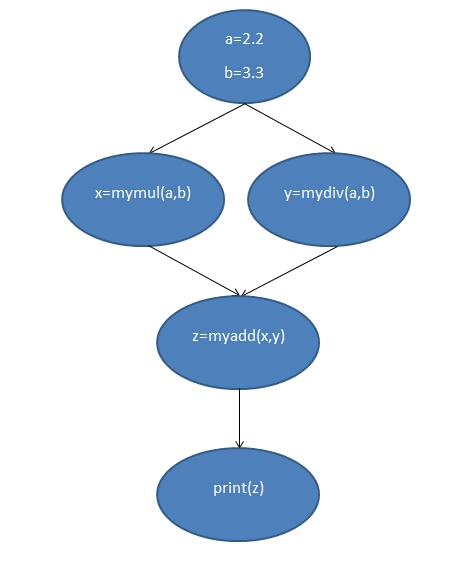
\includegraphics[width=9cm]{15_N_Zaitsev_fig1}
  \caption{~}
  \label{N:Zaitsev:fig1}
\end{figure}
\end{center}

\begin{lstlisting}[language=Python,caption={~},label={NZ:lst3}]
from pycompss.api.task import task	     # Import @task decorator
from pycompss.api.parameter import *	     # Import parameter metadata for the @task decorator
from pycompss.api.api import compss_wait_on  # Import synnchronization function
@task(x=IN, y=IN, returns=float)
def mymul(x, y):
    return x * y
@task(x=IN, y=IN, returns=float)
def myadd(x, y):
    return x + y
@task(x=IN, y=IN, returns=float)
def mydiv(x, y):
    return x/y
if __name__ == '__main__':
    a = 2.2
    b = 3.3
    z = myadd(mymul(a, b), mydiv(a, b))
    z = compss_wait_on(z)
    print(z)
>runcompss abfc.py
[  INFO] Using default execution type: compss
[  INFO] Using default location for project file: /opt/COMPSs/Runtime/configuration/xml/projects/default_project.xml
[  INFO] Using default location for resources file: /opt/COMPSs/Runtime/configuration/xml/resources/default_resources.xml
[  INFO] Inferred PYTHON language\end{verbatim}\begin{verbatim}----------------- Executing abfc.py --------------------------\end{verbatim}\begin{verbatim}WARNING: COMPSs Properties file is null. Setting default values
[(660)    API]  -  Starting COMPSs Runtime v2.5.rc1907 (build 20190702-1710.rb9d4035fbe39f8f3d692d485d359964971080cc0)
7.92666666667
[(4601)    API]  -  Execution Finished\end{lstlisting}
Let us consider the additional lines of the program prepared for exe\-cution by the COMPSs system. The \verb@from ... import ...@ directive describes the import of additional external facilities of the COMPSs system. The \verb@@task (...)@ decorator annotates the functions by specifying input parameters using the \verb@IN@ descriptor and the type of return value using the \verb@returns@ keyword. An expression for the conditional compi\-lation of the main program \verb@if __name__ == '__main__':@ was also added, as well as a call to the synchronization function \linebreak \verb@compss_wait_on (z)@ before printing the result \verb@z@. To run the program, we use the special command \verb@runcompss@.

Additional features of COMPSs, such as visualization of actual graphs of information connections, specification of cluster equipment, and project structure were left beyond the scope of this paper.

\subsection*{4. Conclusions}

The article presents a case study of the basic principles of programs parallelization in the system COMPSs on an example of calculating the arithmetic expression. In essence, it is necessary to add only one additional decoration line for each function declared in the program. Further program parallelization is performed automatically.

Comparisons of COMPSs efficiency with the traditional parallel programming technology such as MPI/OpenMP are rather vague at the present time. That is why the author invites submissions of applied software for various domains which is represented in both variants: a) a conventional program; b) a parallel program in MPI or (and) OpenMP. Comparisons of the obtained benchmarks for 3 cases: 1) conventional; 2) MPI/OpenMP; 3) COMPSs, -- will be reported to the next conference.

\subsection*{Literature}

\begin{thebibliography}{9}
\bibitem{bib1} {COMPSs source code \url{https://github.com/bsc-wdc/compss}}
\bibitem{bib2} {COMP Superscalar, an interoperable programming framework, SoftwareX, Volumes 3–4, December 2015, Pages 32–36, Badia, R. M., J. Conejero, C. Diaz, J. Ejarque, D. Lezzi, F. Lordan, C. Ramon-Cortes, and R. Sirvent, DOI: 10.1016/j.softx.2015.10.004}
\bibitem{bib3} {PyCOMPSs: Parallel computational workflows in Python, Enric Tejedor, Yolanda Becerra, Guillem Alomar, Anna Queralt, Rosa M. Badia, Jordi Torres, Toni Cortes, Jesús Labarta,  IJHPCA 31(1): 66-82 (2017), DOI: 10.1177/1094342015594678}\end{thebibliography}
\end{document}
